% Checkpoint 1, Group 4. Based on the supplied SimplePlus blank template.
% Build: latexmk -pdf -outdir=_build main.tex
\documentclass[aspectratio=169,xcolor=dvipsnames]{beamer}
\usetheme{SimplePlus}
\usepackage[T1,T5]{fontenc}
\usepackage[utf8]{inputenc}
\usepackage{graphicx,booktabs,array,tabularx,listings,hyperref}
\usepackage{pgfpages}
\graphicspath{{figs/}}
\setbeamertemplate{navigation symbols}{}
\setbeamertemplate{footline}{\hfill\insertframenumber\,/\,\inserttotalframenumber\hspace{1em}\vspace{0.5em}}
\setbeamerfont{frametitle}{size=\Large,series=\bfseries}
\setbeamerfont{title}{size=\LARGE,series=\bfseries}
\setbeamerfont{subtitle}{size=\normalsize,series=\bfseries}
\setbeamerfont{block title}{size=\normalsize,series=\bfseries}
\setbeamerfont{block body}{size=\normalsize}
\setbeamerfont{itemize/enumerate body}{size=\normalsize}
\newcommand{\source}[1]{\par\vfill{\tiny\color{gray}#1}}
\newcommand{\keyline}[1]{\par\medskip{\large\color{DarkBlue}\bfseries #1}\par}
\newcommand{\vnote}[1]{\note{\fontencoding{T5}\selectfont #1}}
\lstset{basicstyle=\ttfamily\small,columns=fullflexible,keepspaces=true,
  showstringspaces=false,frame=none,breaklines=true,aboveskip=5pt,belowskip=5pt}
\ifdefined\PRESENTNOTES
  \setbeameroption{show notes on second screen=right}
\fi

\title{ConfigStream}
\subtitle{Scalable Configuration Change Storage\\and Streaming Analytics}
\author{\texorpdfstring{\normalsize Phạm Công Hoàng \quad Lê Tiến Hợp\\[3pt]
  Mai Vũ Hoàng \quad Nguyễn Đức Dũng}{Phạm Công Hoàng, Lê Tiến Hợp, Mai Vũ Hoàng, Nguyễn Đức Dũng}}
\institute{Group 4 \enspace $\cdot$ \enspace Big Data Storage \& Processing}
\date{First milestone checkpoint \enspace $\cdot$ \enspace 26 October 2026}

\begin{document}

% 1 — Title
\begin{frame}
  \vspace*{-2.0em}
  \titlepage
  \vnote{Khoảng 25 giây. Chào thầy và các bạn. Nhóm 4 trình bày ConfigStream, hệ thống lưu trữ và phân tích thay đổi cấu hình. Buổi checkpoint này tập trung vào bài toán, dữ liệu, kiến trúc và những phần nhóm đã triển khai được. Chưa trình bày như một sản phẩm đã hoàn thiện hoặc đã chứng minh khả năng mở rộng.}
\end{frame}

% 2 — One concrete problem
\begin{frame}[fragile]{The problem: configuration changes over time}
  \begin{columns}[T,onlytextwidth]
    \begin{column}{.47\textwidth}
      \begin{block}{Router configuration: version 10}
\begin{lstlisting}
hostname router-001
logging enabled
telnet disabled
\end{lstlisting}
      \end{block}
    \end{column}
    \begin{column}{.47\textwidth}
      \begin{alertblock}{Version 11}
\begin{lstlisting}
hostname router-001
logging disabled
telnet enabled
\end{lstlisting}
      \end{alertblock}
    \end{column}
  \end{columns}
  \vspace{.5cm}
  \keyline{What changed, when, and on which asset?}
  A current configuration file alone cannot answer all three.
  \source{Illustrative input from the executable demo: processing/demo.py.}
  \vnote{Khoảng 45 giây. Mở đầu bằng ví dụ cụ thể: cùng một router nhưng phiên bản sau tắt logging và bật telnet. Đây là dữ liệu minh hoạ do nhóm tạo, không phải sự cố thực tế. Nếu chỉ giữ file hiện tại, ta không biết thay đổi xảy ra lúc nào và khác phiên bản trước ra sao. Nhóm muốn lưu lịch sử và chỉ ra phần thay đổi thay vì chỉ giữ trạng thái cuối cùng.}
\end{frame}

% 3 — Product intent
\begin{frame}{What ConfigStream provides}
  \vspace{.55cm}
  \centering
  
\includegraphics[width=\linewidth,height=3.25cm,keepaspectratio]{goals.png}
  \vspace{.55cm}
  \begin{flushleft}
  \keyline{A searchable history of configuration changes}
  One asset ID links its versions, differences and alerts.
  \end{flushleft}
  \source{Implemented contracts: schemas/; processing/; api/routes/documents.py.}
  \vnote{Khoảng 35 giây. Giải thích ba việc hệ thống làm: lưu phiên bản đã được chấp nhận, so sánh các phiên bản và tra cứu lịch sử cùng cảnh báo theo rule. Asset là đối tượng như router hoặc một file cấu hình. ID của asset giúp nối lịch sử lại với nhau. Cảnh báo là kết quả rule, không đồng nghĩa với một sự cố bảo mật đã được xác nhận.}
\end{frame}

% 4 — The one technical idea to remember
\begin{frame}{Late arrivals should not create the wrong diff}
  \centering
  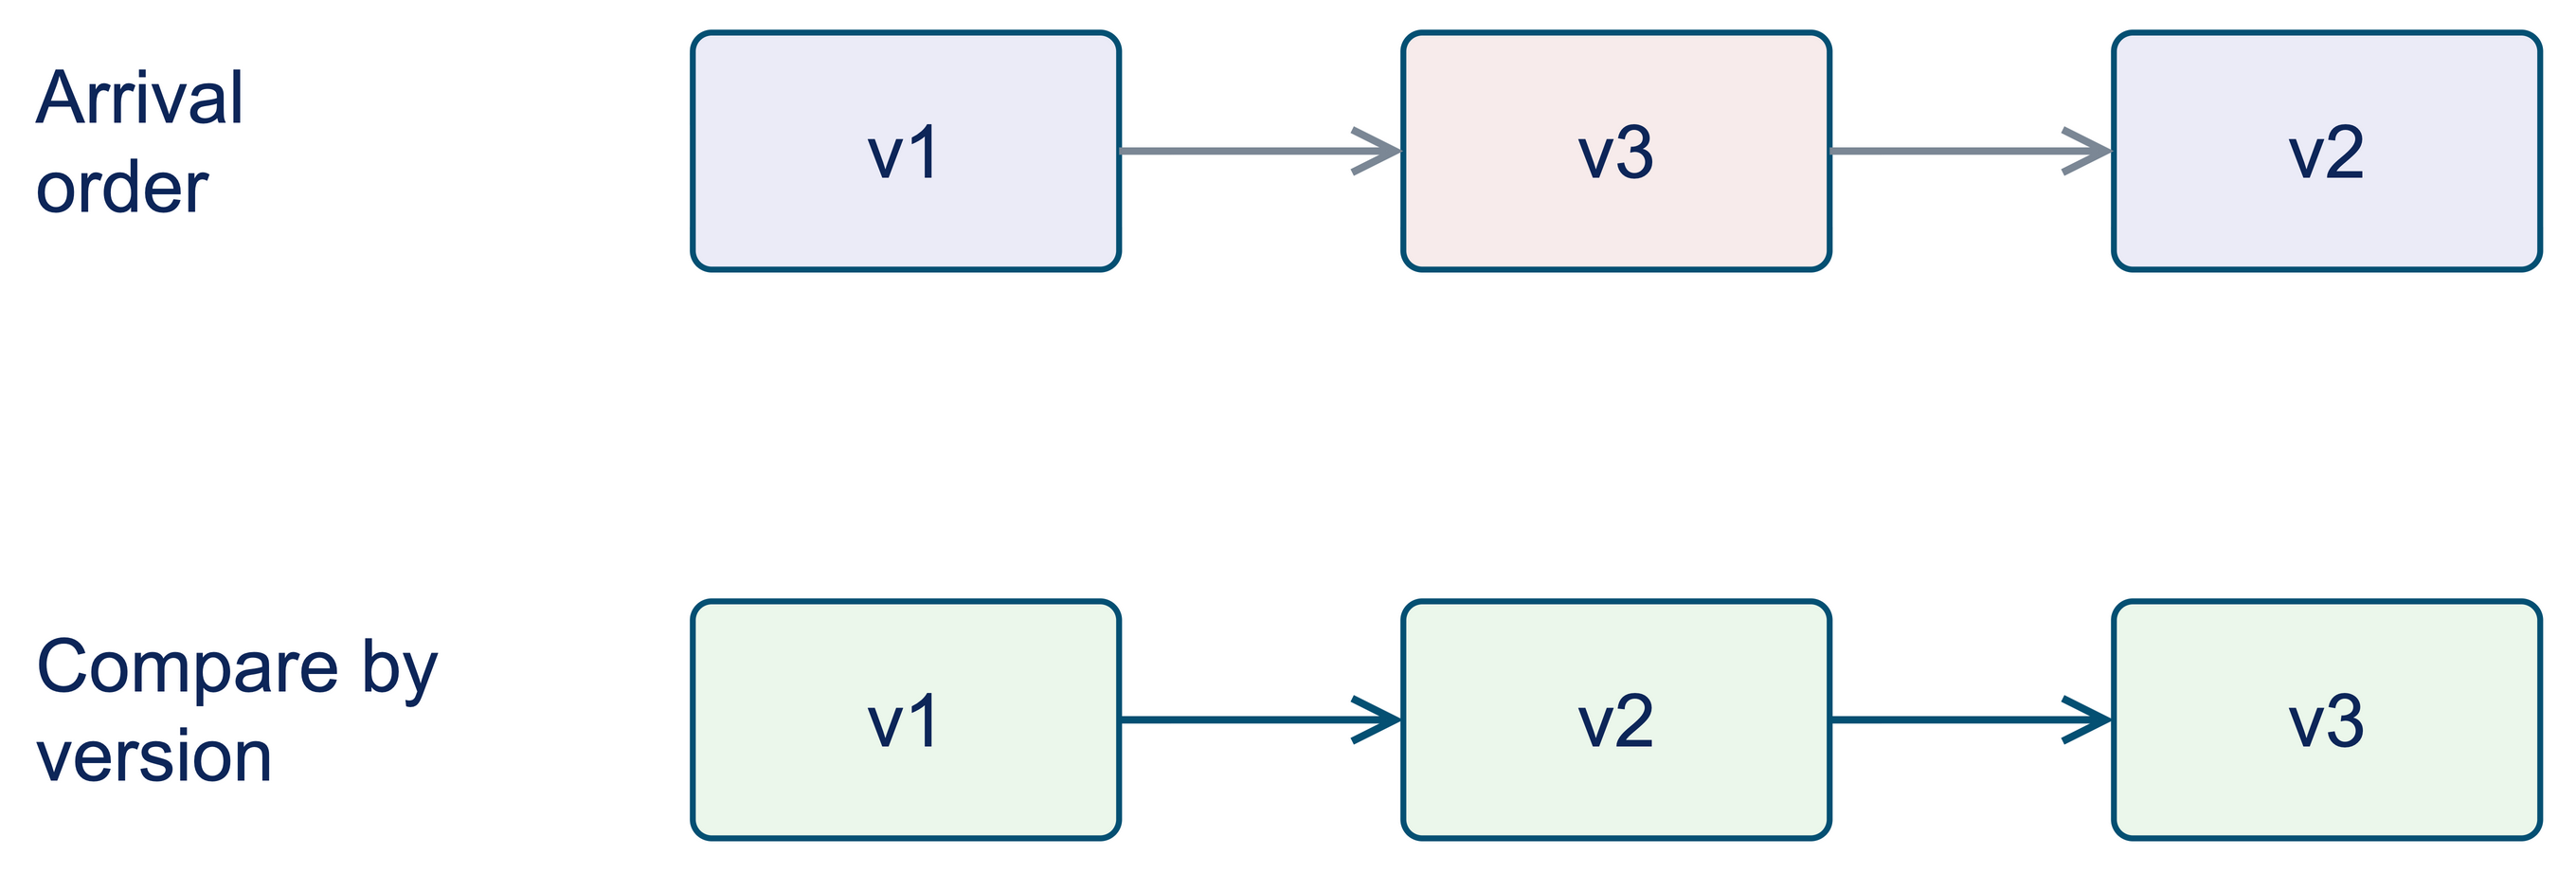
\includegraphics[width=.91\linewidth,height=4.25cm,keepaspectratio]{version-order.png}
  \begin{flushleft}
  Compare \textbf{v1 $\rightarrow$ v2} and \textbf{v2 $\rightarrow$ v3}, once both endpoints are available.
  \end{flushleft}
  \source{processing/state.py; spark/streaming/stateful.py. Online repair is bounded by retained state.}
  \vnote{Khoảng 55 giây. Chỉ vào hàng trên: dữ liệu có thể đến theo thứ tự 1, 3, 2. Nếu so sánh theo thứ tự đến, ta sẽ tạo cặp 1 sang 3 và bỏ qua phiên bản 2. Hàng dưới là cách nhóm xử lý: giữ các phiên bản theo asset và chỉ tạo diff giữa các phiên bản liền kề. Nếu 2 đến khi state còn giữ được 1 và 3 thì tạo đủ hai cặp đúng. State có giới hạn lưu giữ, nên không hứa sửa được mọi dữ liệu đến muộn vô hạn.}
\end{frame}

% 5 — System architecture
\begin{frame}{System architecture}
  \centering
  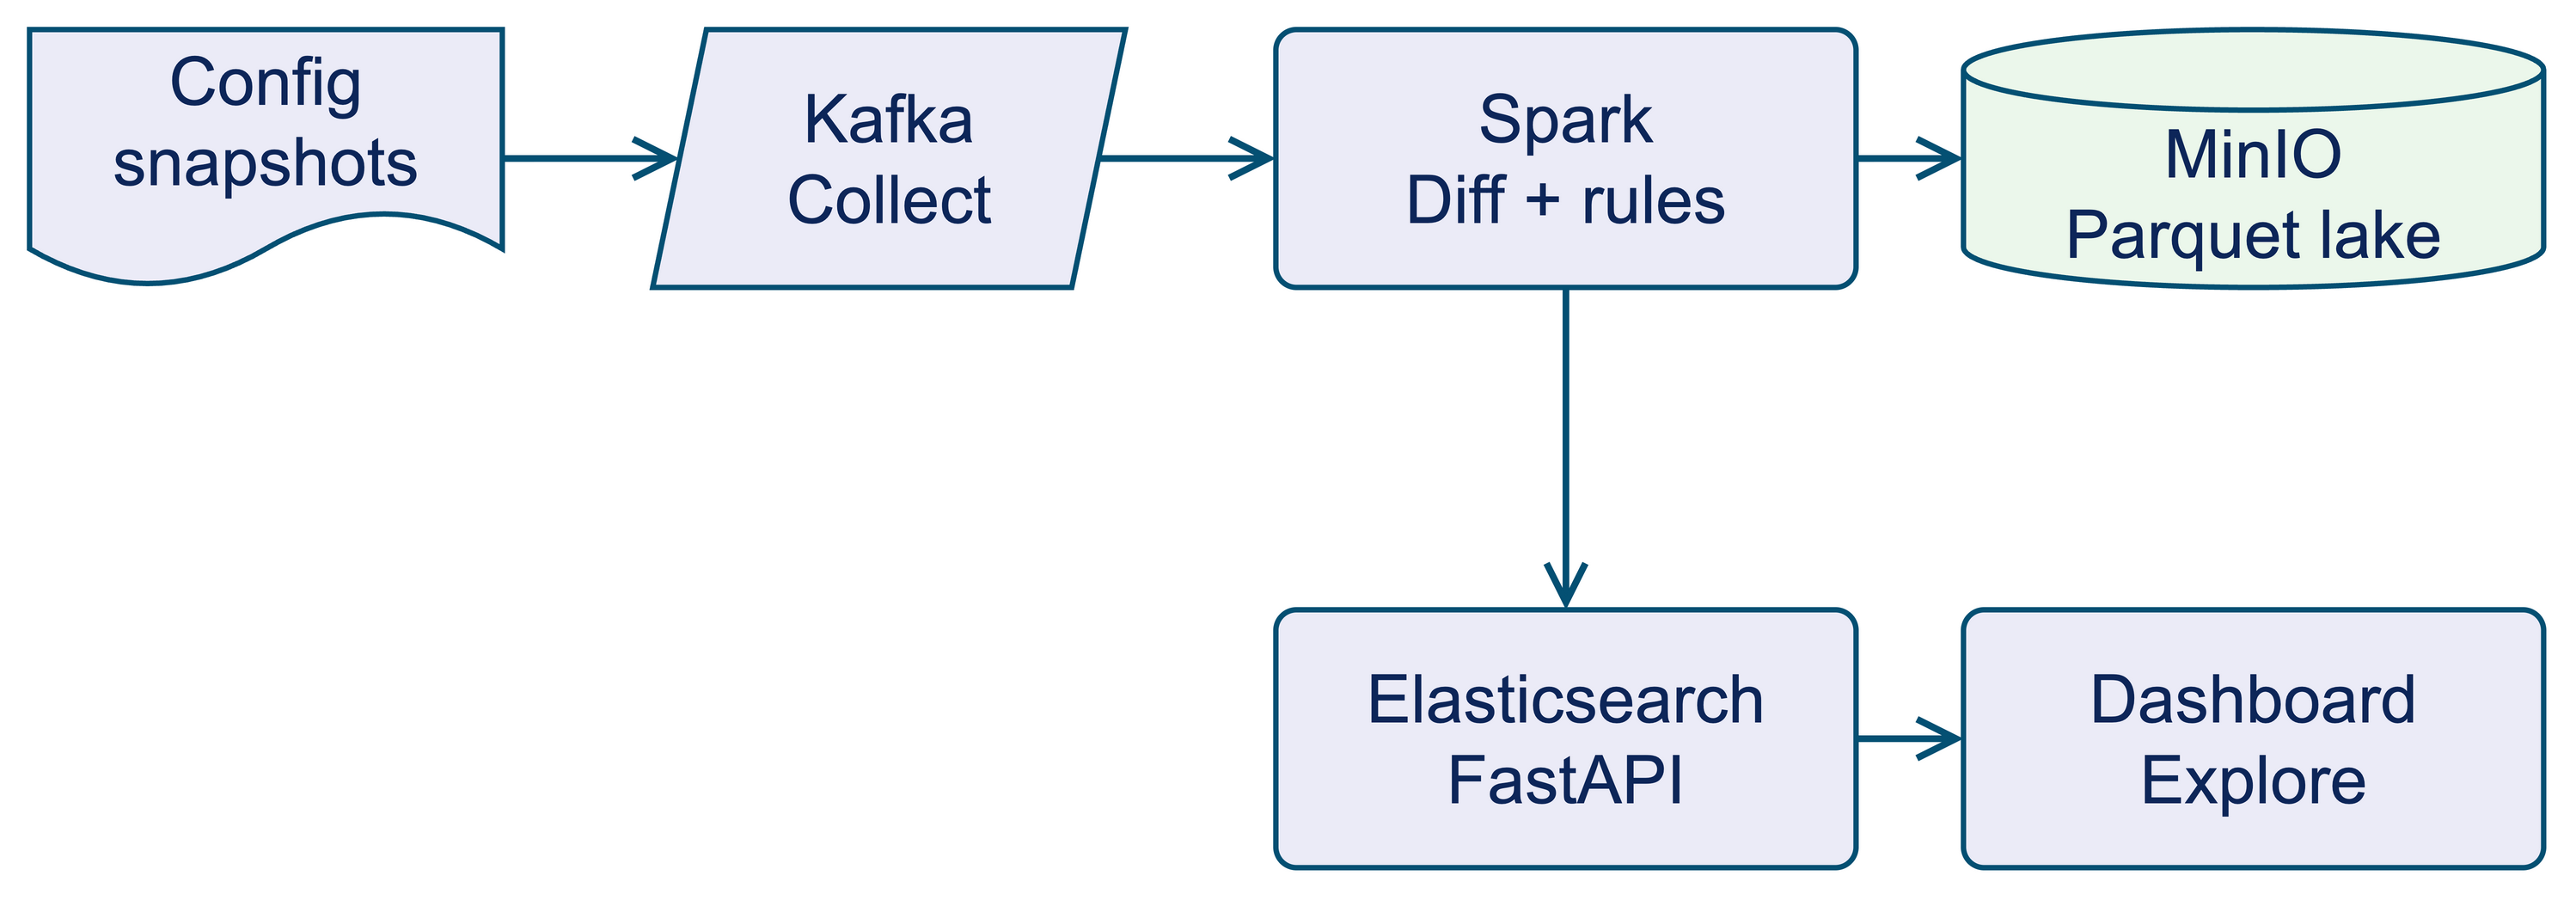
\includegraphics[width=.97\linewidth,height=4.55cm,keepaspectratio]{architecture.png}
  \begin{flushleft}\small
    Parquet keeps the durable history. Search and the dashboard provide read access.\\
    Historical Spark analytics reads the committed Parquet datasets.
  \end{flushleft}
  \source{Configuration path: spark/streaming/outputs.py; analytics/main.py; api/; frontend/.}
  \vnote{Khoảng 65 giây. Đi theo mũi tên: snapshot đi qua Kafka, Spark chuẩn hoá và so sánh phiên bản, rồi ghi lịch sử vào MinIO dưới dạng Parquet. Nhánh bên dưới ghi metadata vào Elasticsearch, FastAPI cung cấp API và dashboard hiển thị. Lịch sử Parquet là dữ liệu gốc để đọc lại; search là lớp phục vụ truy vấn. Trong code, lake được ghi trước search. Sơ đồ rút gọn đường cấu hình; các bộ dữ liệu RPKI, RIS, DNS có pipeline riêng và không bị ép qua bộ so sánh cấu hình này. Nếu thầy hỏi analytics batch, nó đọc Parquet đã commit.}
\end{frame}

% 6 — Ready data, with clear units
\begin{frame}{Data is ready for development and replay}
  \begin{columns}[T,onlytextwidth]
    \begin{column}{.40\textwidth}
      {\large\bfseries\color{DarkBlue}Controlled examples}\par\medskip
      A deterministic generator creates snapshots, retries and late arrivals.
      \medskip
      Useful for checking whether the result is correct.
    \end{column}
    \begin{column}{.54\textwidth}
      {\large\bfseries\color{DarkBlue}TerraDS configuration history}\par\medskip
      \renewcommand{\arraystretch}{1.5}
      \begin{tabular}{@{}rl@{}}
        \textbf{6,505} & file histories \\
        \textbf{10,188} & accepted versions \\
        \textbf{3,683} & adjacent version pairs
      \end{tabular}\par
      \medskip
      Public Git history of infrastructure code.
    \end{column}
  \end{columns}
  \vspace{.45cm}
  {\small Large datasets stay outside Git; source manifests and result receipts are versioned.}
  \source{generator/; workloads/results/terrads/history-summary.json. Git changes are not deployment events.}
  \vnote{Khoảng 50 giây. Nhóm có hai loại dữ liệu. Bộ tạo dữ liệu giúp chủ động kiểm tra thứ tự đảo, dữ liệu lặp và các thay đổi biết trước. TerraDS là lịch sử mã hạ tầng từ Git: 6.505 lịch sử file, 10.188 phiên bản và 3.683 cặp liền kề được chấp nhận. Không gọi đây là 10.188 lần triển khai ngoài thực tế. Dữ liệu lớn không đưa hết vào Git; repo giữ nguồn gốc, manifest và kết quả. Nếu được hỏi thêm, nhóm còn có dữ liệu RPKI, RIS và DNS, nhưng hôm nay tập trung đường xử lý cấu hình để dễ theo dõi.}
\end{frame}

% 7 — Visible processing result
\begin{frame}[fragile]{Implemented: differences and rule alerts}
  \begin{columns}[T,onlytextwidth]
    \begin{column}{.48\textwidth}
      \begin{block}{Diff: version 10 $\rightarrow$ 11}
        {\ttfamily\small
          \textcolor{MediumRed}{- logging enabled}\\[3pt]
          \textcolor{MediumRed}{- telnet disabled}\\[3pt]
          \textcolor{MediumBlue}{+ logging disabled}\\[3pt]
          \textcolor{MediumBlue}{+ telnet enabled}}
      \end{block}
    \end{column}
    \begin{column}{.46\textwidth}
      {\large\bfseries\color{DarkBlue}Rules detect}\par\medskip
      \textbf{Logging disabled}\\
      High severity\par\medskip
      \textbf{Telnet enabled}\\
      Critical severity
    \end{column}
  \end{columns}
  \vspace{.55cm}
  Repeated delivery must not invent another logical change.
  \source{processing/demo.py; processing/diff.py; rules/default.yaml; tests/unit/test\_rules.py.}
  \vnote{Khoảng 45 giây. Quay lại ví dụ đầu: output chỉ ra các dòng bị bỏ và thêm. Rule mặc định báo logging bị tắt ở mức high và telnet được bật ở mức critical. Đây là rule minh hoạ đã có trong code, không phải mô hình AI dự đoán. Chuẩn hoá xử lý các khác biệt văn bản được hỗ trợ; không phải parser hiểu mọi ý nghĩa cấu hình. Việc gửi lại cùng snapshot cũng không được tạo thêm thay đổi logic mới.}
\end{frame}

% 8 — Executable repository
\begin{frame}[fragile]{Executable code is available in Git}
  \begin{columns}[T,onlytextwidth]
    \begin{column}{.45\textwidth}
      {\large\bfseries\color{DarkBlue}Repository}\par\medskip
      \begin{tabular}{@{}ll@{}}
        \texttt{generator/} & input data \\[5pt]
        \texttt{processing/} & diff and rules \\[5pt]
        \texttt{spark/} & streaming jobs \\[5pt]
        \texttt{api/} & read API \\[5pt]
        \texttt{frontend/} & dashboard
      \end{tabular}
    \end{column}
    \begin{column}{.49\textwidth}
      \begin{block}{Small demo, no services required}
\begin{lstlisting}
make setup
make processing-demo
\end{lstlisting}
      \end{block}
      \medskip
      \textbf{178 core tests passed}\\
      State logic, diffs and rules\\
      {\small Rechecked on 25 October 2026}
    \end{column}
  \end{columns}
  \source{github.com/kongwoang/ConfigStream; Makefile; tests/unit/test\_state\_logic.py, test\_diff.py, test\_rules.py.}
  \vnote{Khoảng 50 giây. Mở link repo nếu có mạng hoặc chuyển terminal đã chuẩn bị. Hai lệnh trên chạy demo xử lý thuần Python, không cần dựng Kafka hay MinIO. Không dùng demo nhỏ này để nói cả stack đang online. Nhóm vừa kiểm tra 178 test của state logic, diff và rule. CI của revision mã nguồn 3980ce1 đã đạt trước khi thêm slide. Nếu thầy muốn xem thực thi, chạy make processing-demo; phần output chính chính là ví dụ vừa giải thích.}
\end{frame}

% 9 — Recorded integrated evidence, separate from today's small demo
\begin{frame}{A complete local replay has been recorded}
  \vspace{.45cm}
  \centering
  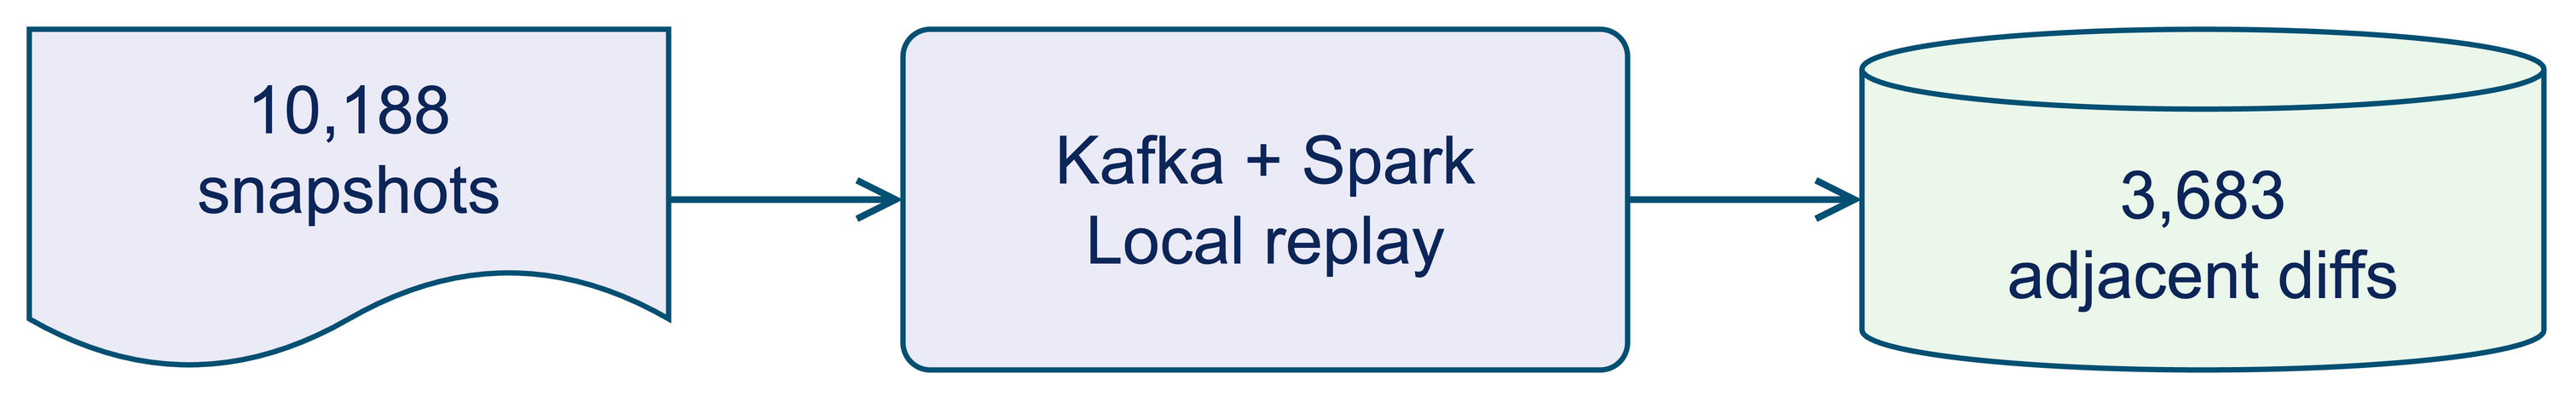
\includegraphics[width=\linewidth,height=3.25cm,keepaspectratio]{replay.png}
  \vspace{.45cm}
  \begin{flushleft}
  \textbf{29.4 MB} of raw and processed Parquet committed.\\[5pt]
  This demonstrates the integrated path on the selected local workload.
  \end{flushleft}
  \source{Recorded acceptance: docs/phase12-acceptance.md. 29,402,997 bytes; not a new replay or a scale benchmark.}
  \vnote{Khoảng 40 giây. Đây là kết quả replay đã được ghi nhận trong repo, không phải lần chạy mới trong buổi thuyết trình. 10.188 snapshot qua đường tích hợp và cho 3.683 diff liền kề. Khoảng 29,4 MB là tổng Parquet raw và processed đã commit. Chỉ kết luận đường tích hợp chạy được trên phạm vi local đã thử; không kết luận Spark nhanh hơn baseline hay hệ thống đã đạt quy mô production. Cấu hình replay lịch sử có retention riêng, khác mặc định demo online.}
\end{frame}

% 10 — Actual application, no mocked live data
\begin{frame}{Dashboard preview}
  \centering
  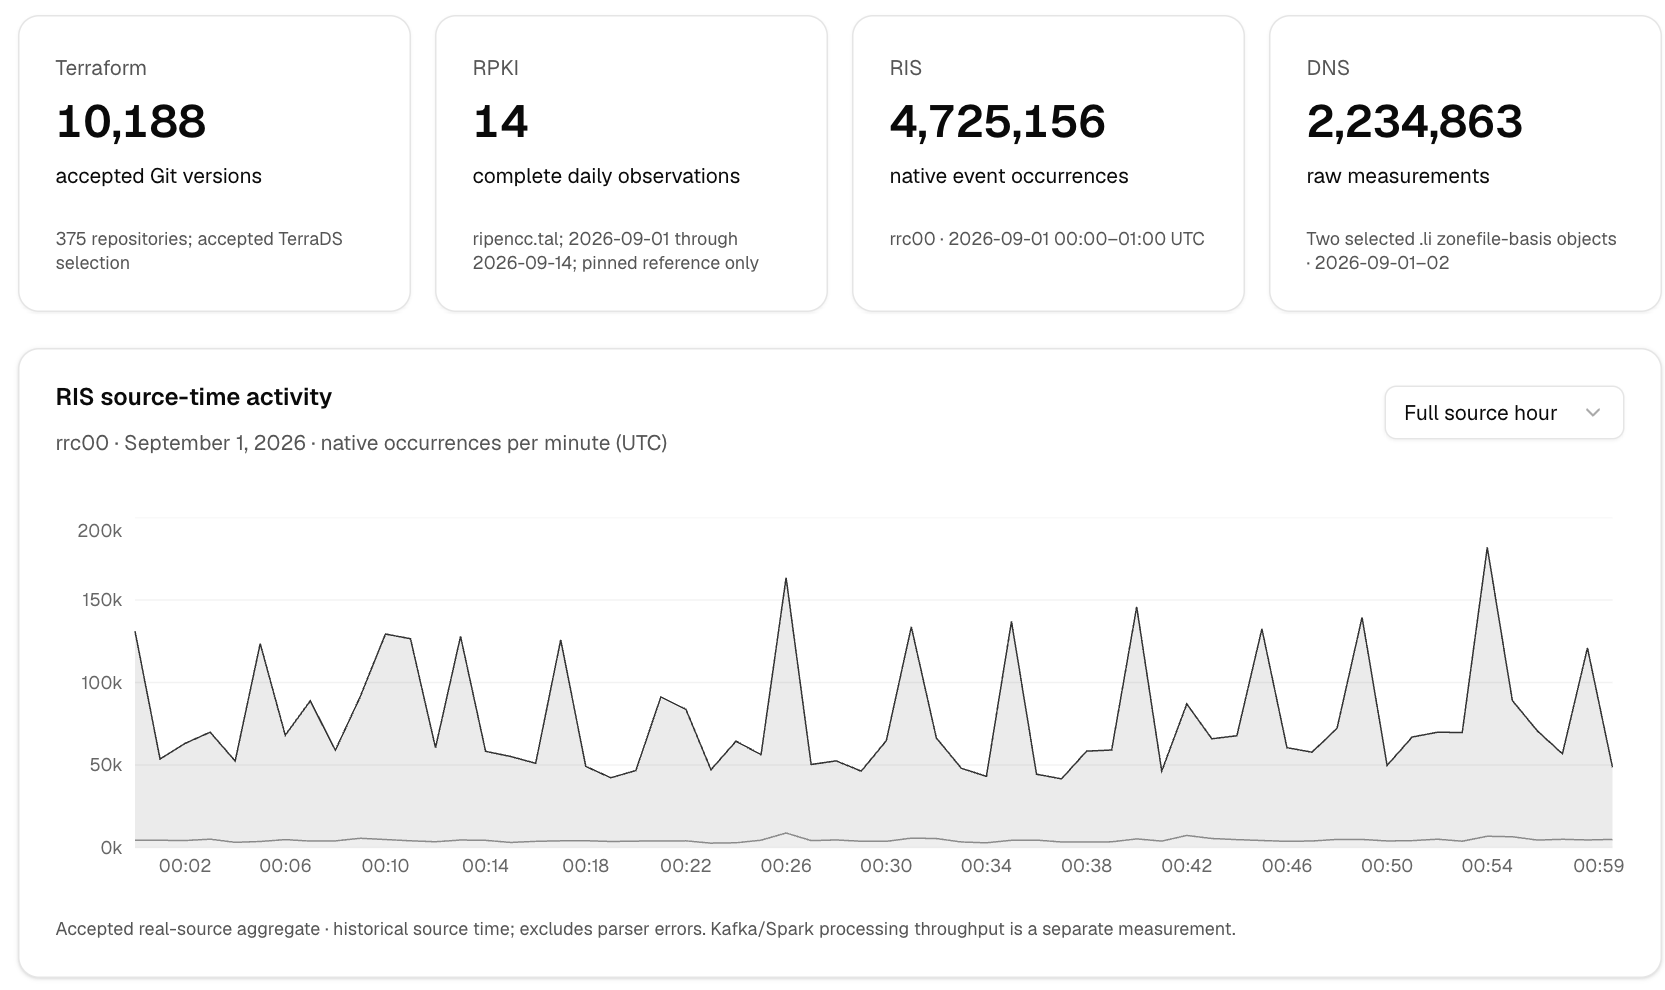
\includegraphics[width=\linewidth,height=5.5cm,keepaspectratio]{dashboard.png}
  \source{Actual frontend captured on 25 October 2026. This overview displays the accepted evidence bundle, not a live replay.}
  \vnote{Khoảng 40 giây. Đây là ảnh giao diện thật được mở từ frontend hiện tại. Trang overview tóm tắt dữ liệu đã được chấp nhận ở các miền. Phần lịch sử cấu hình có API để tra cứu theo asset và thời gian khi backend chạy. Các con số trên ảnh thuộc những đơn vị khác nhau, không cộng lại thành một chỉ số tổng. Ảnh này không chứng minh backend đang chạy trực tiếp trong buổi checkpoint.}
\end{frame}

% 11 — Direct answer to the instructor
\begin{frame}{Checkpoint readiness}
  \renewcommand{\arraystretch}{1.8}
  \begin{tabularx}{\linewidth}{@{}p{.26\linewidth}X@{}}
    \toprule
    \textbf{Requirement} & \textbf{What the group can show} \\
    \midrule
    Git + executable code & Repository, runnable demo and automated tests \\
    Data ready & Controlled inputs, TerraDS history and source manifests \\
    Architecture ready & Kafka, Spark, Parquet, search API and dashboard \\
    \bottomrule
  \end{tabularx}
  \vspace{.45cm}
  \keyline{The core workflow is implemented and demonstrated locally}
  \vnote{Khoảng 40 giây. Trả lời trực tiếp ba yêu cầu thầy đưa ra. Git đã có code chạy được; dữ liệu và manifest đã chuẩn bị; kiến trúc đã có implementation và minh chứng local. Chỉ vào đúng slide trước tương ứng mỗi hàng. Chưa gọi đây là bài hoàn thành cuối kỳ; vẫn cần củng cố demo tích hợp, đo đạc và cách trình bày kết quả.}
\end{frame}

% 12 — Honest next milestone
\begin{frame}{Next milestone}
  \begin{enumerate}\setlength{\itemsep}{.8em}
    \item \textbf{Rehearse the integrated demo}\\
      Start the services, send a change, inspect the stored result.
    \item \textbf{Evaluate larger workloads}\\
      Measure throughput, latency and storage with clear units.
    \item \textbf{Strengthen recovery evidence}\\
      Repeat failure and restart checks for the latest revision.
  \end{enumerate}
  \vspace{.35cm}
  {\small Current evidence is local / single-node; distributed scale and HA remain open.}
  \vfill
  {\large\color{DarkBlue}\bfseries Thank you --- questions?}
  \vnote{Khoảng 40 giây. Ba việc nhóm dự kiến ưu tiên tiếp: diễn tập demo tích hợp từ đầu, mở rộng đánh giá với đơn vị đo rõ ràng và chạy lại kiểm thử phục hồi trên revision mới nhất. Không nói những việc dự kiến này đã hoàn thành. Bằng chứng hiện có chủ yếu local hoặc single-node; chưa chứng minh HA hay horizontal scalability. Kết thúc và mời thầy góp ý về phạm vi dữ liệu và ưu tiên cho milestone tiếp theo.}
\end{frame}

\end{document}
